\chapter{ESP32}

\section{Project Structure}

\section{FaRiLib}
To share common functionality across all nodes, a library called FaRiLib was
created. Its goal is to provide a common interface for all nodes to use, such as
a common way to handle incoming messages and to send messages to the bridge node. 
\par\vspace{0.5em}
It's placed in the \texttt{SW-ESP/globalLibs} directory and should be included in
every node project placed in the \texttt{SW-ESP} directory.
    \subsection{Library Structure}
        \begin{minipage}{0.48\textwidth}
            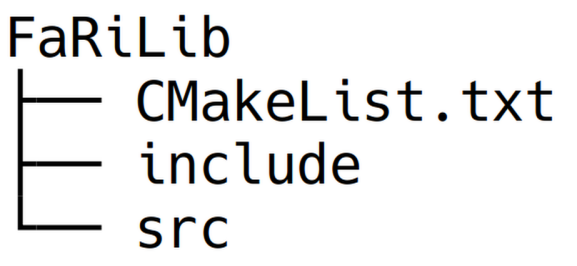
\includegraphics[width=0.8\linewidth]{assets/FaRiLibStructure.png}
            \label{fig:farilib_structure}
        \end{minipage}%
        \begin{minipage}{0.48\textwidth}
            \raggedright
            \begin{itemize}
                \item \textbf{CMakeLists.txt}: The CMake configuration file for the 
                library.
                \item \textbf{src/}: The source files of the library.
                \item \textbf{include/}: The header files of the library.
            \end{itemize}
        \end{minipage}
        \subsubsection{CMakeLists.txt}
        For the inclusion to work properly, a \texttt{CMakeLists.txt} file is
        necessary. It should contain the following lines: 
    \begin{lstlisting}[style=cppCode]
    project(FaRiLib)

    include_directories(include)

    set(SOURCE_FILES
            src/*
    )
    \end{lstlisting}
        In combination with the configuration done in section \ref{sec:farilib_include},
        this enables an include as simple as \texttt{\#include <FaRiLib.h>} in all
        node projects.

    \subsection{ESP NOW}

\section{Project Configuration}

    \subsection{platformio.ini}
    Every project in PlatformIO requires a \texttt{platformio.ini} file. This file
    contains all the necessary information for the build process. Its content may
    vary depending on the project, but for this Smart Home System, the following
    configuration stays consistent:
    \begin{lstlisting}[style=cppCode]
    [env:<BOARDNAME>]
    platform = espressif32
    board = <BOARDNAME>
    framework = arduino
    \end{lstlisting}
    The \texttt{<BOARDNAME>} should be replaced with the name of the board used
    for the Node, for example, \texttt{esp32-s3-devkitm-1} for the ESP32-S3 or
    \texttt{esp32c3-devkitm-1} for the ESP32-C3.

        \subsubsection{platform}
        The \texttt{platform} key specifies the platform to build for. Due to the
        fact that the networking is dependent on ESP-NOW, this will most likely be
        \texttt{espressif32} or \texttt{espressif8266} depending on the 
        microcontroller.
        
        \subsubsection{framework}
        The \texttt{framework} key specifies the framework to use. All, for this 
        thesis developed nodes, are based on the Arduino framework, however, other
        frameworks for the ESP32 are available, such as ESP-IoT-Development-Framework
        (ESP-IDF for short) maintained by Espressif and designed exclusively for the 
        ESP32.
        
        Other \textbf{more specific 
        configurations} that are necessary will be discussed in the \textbf{following 
        sections}.

    \subsection{Enabling the Serial Monitor}
    While reading the serial monitor is not necessary for functionality, it is a
    useful tool for debugging. For older ESP32 boards no additional configuration 
    should be necessary, newer boards however, such as the \texttt{ESP32-S3} and the 
    \texttt{ESP32-C3}, require the following \texttt{build\_flags}: 
    \begin{lstlisting}[style=cppCode]
    build_flags =
    -DARDUINO_USB_MODE=1
    -DARDUINO_USB_CDC_ON_BOOT=1
    \end{lstlisting}
    After that, the monitor speed can be set as well:
    \begin{lstlisting}[style=cppCode]
    monitor_speed = 9600
    \end{lstlisting}
    The baud rate can be adjusted to any desired value as long as the clock rate
    of the board supports it, but note that it should match the baud rate set in 
    the code. Common values are 115200 or 9600 on older boards.

    \subsection{Including FaRiLib} \label{sec:farilib_include}
    Due to the fact that the FaRilib library shoul be used across all nodes, it is
    placed inside the \texttt{SW-ESP} directory and included in all node-projects.
    To add the directory to the include path, the following lines should be added to
    the \texttt{platformio.ini} file:
    \begin{lstlisting}[style=cppCode]
    lib_extra_dirs =
        ../globalLibs
    \end{lstlisting}
    Note that the path is relative, meaning it needs to be adjusted should the project
    be places outside the \texttt{SW-ESP} directory.